
\section{Optics and Wave Phenomena}
(such as wave properties, superposition,
interference, diffraction,
geometrical optics, polarization,
Doppler effect)

\subsection{Wave properties}

\Table{
\hline

The wave equation & $\dfrac{\partial^2 u}{\partial t^2} = c^2 \nabla^2 u.$

\\ \hline

General solution & $u(x,t) = A \sin(kx - \omega t) + B \cos(dx - \omega t).$

\\ \hline

$c$ & $c = \omega / k$

\\ \hline
}

%%%%

\Table{
\hline

\textbf{General wave function} $f(x,t,k,\omega) = $ & $A \sin (kx \pm \omega t) $

\\ \hline

wave function $f(x,t,\lambda,T) = $ & $A \sin 2\pi (\dfrac{x}{\lambda} \pm \dfrac{t}{T})$

\\ \hline
}

%%%%

\Table{
\hline

Amplitude & $A$

\\ \hline

Period & $T$

\\ \hline
}

%%%%

\Table{
\hline

Direction &

\MiniPg{.7}{ The $\sin$ function preserves a sine wave form as it traverses $x$ and $t$. The argument must remain constant:  $kx \pm \omega t = constant$. In order to preserve this, must $x$ increase or decrease as $t$ increases? Depends on the $\pm$ }

\\ \hline
}

%%%%

\Table{
\hline

$k = $	& $k = 2\pi / \lambda $

\\ \hline

$\omega = $	& $= \omega = 2 \pi f = 2 \pi / T $

\\ \hline
}

%%%%

\Table{
\hline

Phase velocity	& $v_{ph} = \omega / k  = \lambda / T$

\\ \hline

Group velocity	& $v_g = \dfrac{\partial \omega}{\partial k} $

\\ \hline
}

%%%%%%%%%%%%%%%%%%%%%%%%%%%%%%%%%%%%%%%%%%%

\subsection{Waves on a string}
\Table{
\hline

Characteristic impedance of a string & $Z = \mu c$ where $\mu$ is the mass \\
							& per unit length \& c is the wave speed.

\\ \hline
}

If you want to be super in the know about transverse waves on strings, check this out: \url{http://www.people.fas.harvard.edu/~djmorin/waves/transverse.pdf }

%\subsection{Superposition}


%%%%%%%%%%%%%%%%%%%%%%%%%%%%%%%%%%%%%%

\subsection{Interference}
\Table{
\hline

\MiniPg{.4}{

Michelson Interferometer equation relating distance (moved perhaps), number of fringes, and wavelength.

}

&

\MiniPg{.6}{
$2d = m \lambda$, where $m$ is the number of fringes. The factor of 2 comes from the fact that the light crosses the same distance twice. See GR9277 \#96 for an interesting problem.
}
\\ \hline
}

%%%%%%%%%%%%%%%%

\subsubsection{Two waves at the same speed}
\Table{
\hline

Sine waves in  & Same $\rightarrow$ interference. Opposite $\rightarrow$ standing. \\
same/opp. direction & 

\\ \hline

Constructive if & $\phi_1 = \phi_2$ \\
Destructive if & $|\phi_1 - \phi_2| = \pi$

\\ \hline
}

%%%%

\Table{
\hline

Standing wave  & $u(x,t) = A \sin(kx - \omega t) + A \sin (kx + \omega t) $ \\
equation					& $= 2 A \sin(kx)\, \cos(\omega t).$

\\ \hline
}

%%%%%

\Table{
\hline

Condition for nodes & $u(x,t) = 0 \,\, \Rightarrow \,\, kx = n\pi$

\\ \hline

Condition for antinodes & $u(x,t) = \textrm{max.} = 2A  \,\, \Rightarrow \,\, kx = \pi/2 + n\pi$

\\ \hline
}

%%%%

\Table{
\hline

Condition for beats & Same direction, different frequency

\\ \hline

Equation for beats & $u(x,t) = A \sin(k_1x - \omega_1 t) + A \sin (k_2x + \omega_2 t) $ \\
			& $=2A \sin \Big[ \dfrac{(k_1 + k_2)x}{2} - \dfrac{(\omega_1 + \omega_2)t}{2} \Big]\cos \Big[ \dfrac{(k_1 - k_2)x}{2} - \dfrac{(\omega_1 - \omega_2)t}{2} \Big]$
			
\\ \hline

Beat frequency & $\omega_{beat} = |\omega_1 - \omega_2|$

\\ \hline
}

%%%%%%%%%%%%%%%%%%%%%%%%%%%%%%%%

\subsubsection{Holography}
\Table{
\hline

Holographs & \begin{minipage}{.6\textwidth}
 encode the light field as an interference pattern, recording phase and amplitude.
 \end{minipage}
 
 \\ \hline
}

%%%

\Table{
\hline
 
 Holograph construction
 
 &
 
 \begin{minipage}{.5\textwidth}
      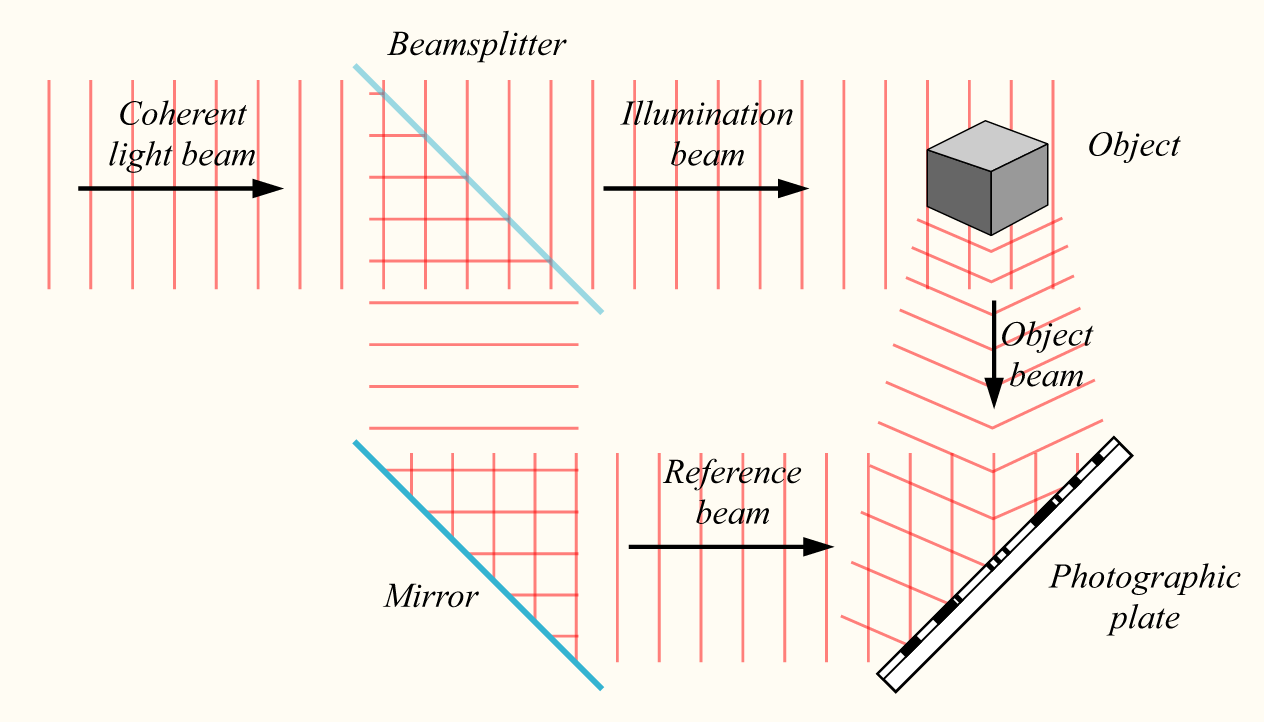
\includegraphics[width=\linewidth, height=45mm]{images/HoloConstruct.png}
      
       \end{minipage}
       
\\ \hline
}

%%%%

\Table{
\hline

 Holograph construction
 
 &
 
 \begin{minipage}{.3\textwidth}
      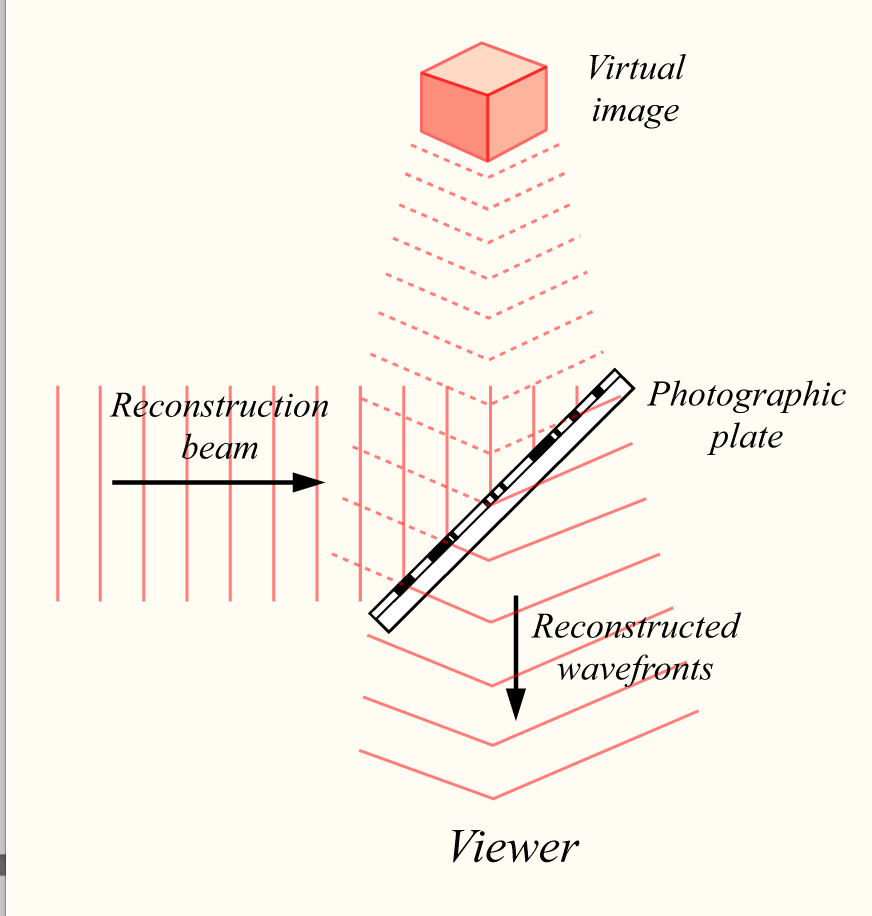
\includegraphics[width=\linewidth, height=45mm]{images/HoloRecon.png}
      \tiny \url{https://en.wikipedia.org/wiki/Holography}
       \end{minipage}
       
\\ \hline
}

%%%%%%%%%%%%%%%%%%%%%%%%%%%%%%%%%%%%%%%%%%%%

\subsection{Refraction}
\center
\begin{figure}[htbp]
    \begin{center}
	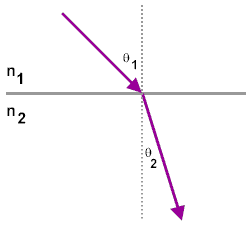
\includegraphics[width=60mm]{images/IncidentRefracted.png}
    \end{center}
    \linespread{1} 
	\caption[Incident and refracted rays]{
	\tiny http://vignette2.wikia.nocookie.net/schools/images/4/4c/097b8946-3139-4ea1-8573-05128eb66b29.gif/revision/latest?cb=20060612224020

	}
\label{IncRefRays}
\end{figure}

%%%%%%

\Table{
\hline

Index of refraction & $n \equiv \dfrac{c}{v}$

\\ \hline
}

%%%%

\Table{
\hline

I.o.R. and wavelengths

&

\MiniPg{.6}{
\center

$n = \dfrac{\lambda_0}{\lambda}$

Where $\lambda_0$ is the wavelength in vacuum and $\lambda$ is the wavelength in medium.
}
 
\\ \hline
}

%%%%

\Table{
\hline

$n$ can be $<1$ if & the phase velocity is greater than c.

\\ \hline

Snell's law & $n_i \sin \theta_i = n_f \sin \theta_f$ 

\\ \hline
}

\Table{
\hline

Draw with $n_2 > n_1$ and $n_1 > n_2$    & \begin{minipage}{.4\textwidth}
      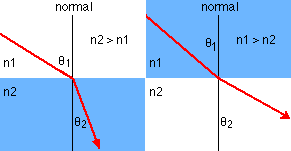
\includegraphics[width=\linewidth, height=30mm]{images/optic-snell.png}
      \tiny \url{http://www.astrosurf.com/luxorion/Physique/optic-snell.gif}
    \end{minipage}

\\ \hline
}

%%%%

\Table{
\hline

Condition for total internal reflection & $\dfrac{n_i \sin \theta_i}{n_f} > 1$

\\ \hline

Critical angle & $\theta_c = \theta_i = \arcsin \BigP{\dfrac{n_2}{n_1}}$

\\ \hline
}

%%%%

\Table{
\hline

Dispersion and general trend & $n(\lambda)$, as $\lambda \Uparrow, n \downarrow$

\\ \hline
}

%%%%

\Table{
\hline

Fraction of light reflected $R$ & $R = \Big( \dfrac{n_1 - n_2}{n_1 + n_2} \Big)^2$

\\ \hline

Fraction of light transmitted & $T = 1 - R = \dfrac{4 n_1 n_2}{(n_1 - n_2)^2 }$


\\ \hline
}

%%%%%%%%%%%%%%%%%%%%%%%%%%%%%%%%%%%%%%%

\subsubsection{Thin Films}
\Table{
\hline
\begin{minipage}{.3\textwidth}
Soap/oil film constructive and destructive interference
\end{minipage}

&

\MiniPg{.6}{

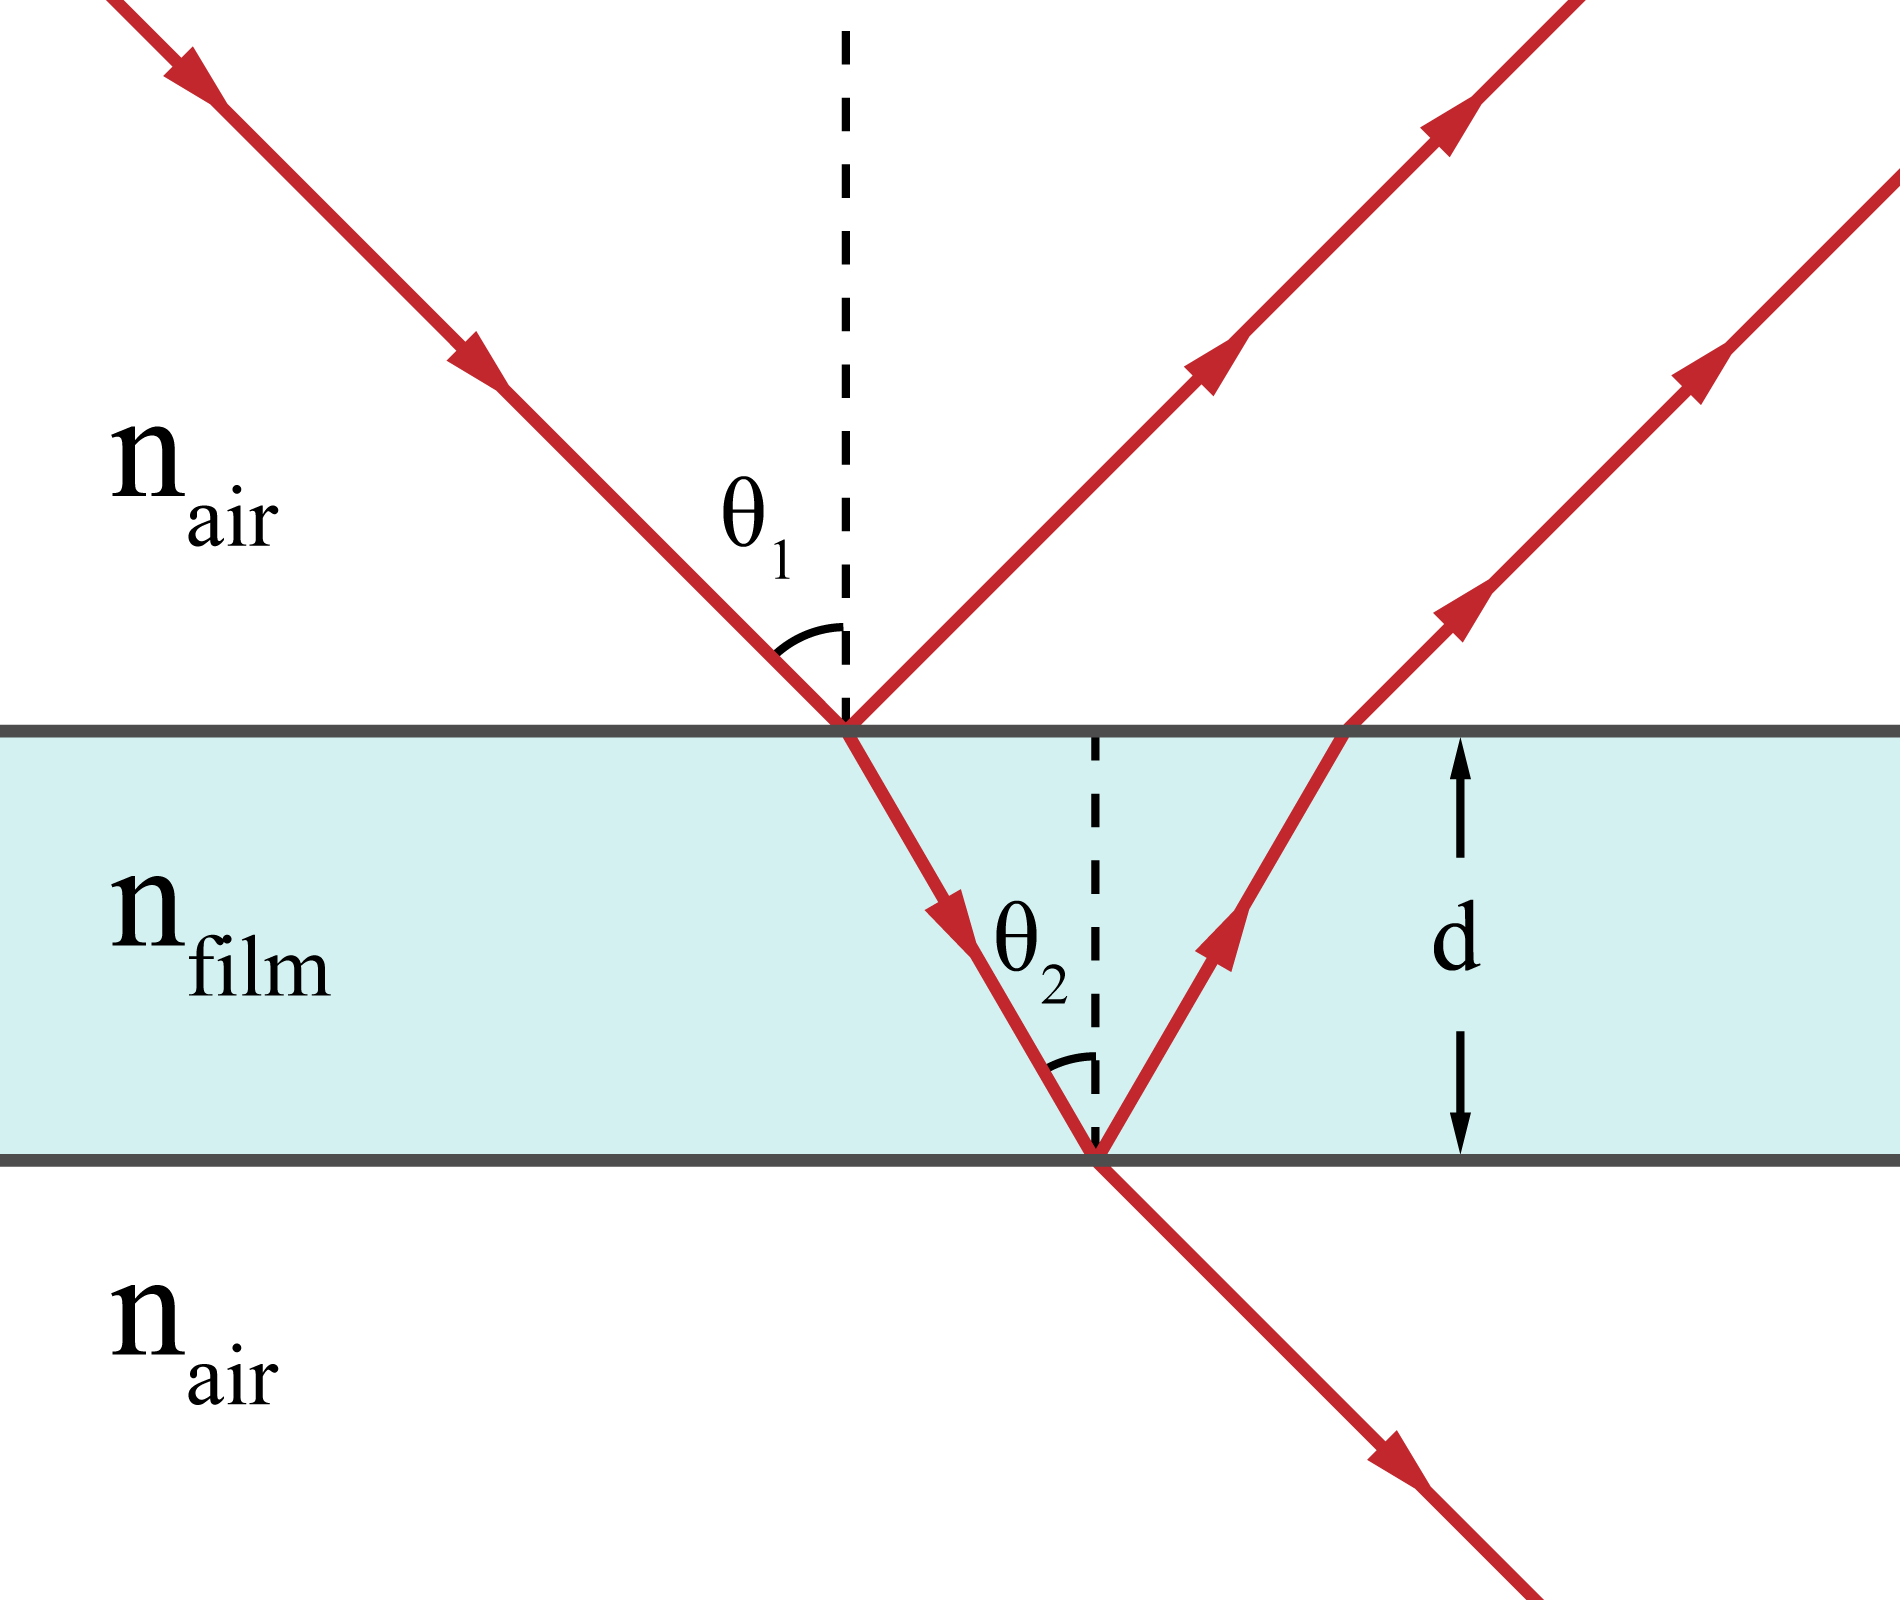
\includegraphics[width=55mm, height=40mm]{images/ThinFilmSoap.png}
      \tiny \url{https://en.wikipedia.org/wiki/Thin-film_interference}
      
      \large
      $n_{film} > n_{air}$. Also, the bottom air can be swapped with a water section, in which case $n_{film} > n_{water} >  n_{air}$, and the following equations still hold.
      
      Constructive: $2n_{film}d \cos(\theta_2) = (m-\frac{1}{2}) \lambda$
      
      Destructive: $2n_{film}d \cos(\theta_2) = m \lambda$
      

}
\\ \hline
}

%%%%

\Table{
\hline

\begin{minipage}{.3\textwidth}
Coating film constructive and destructive interference
\end{minipage}

&

\begin{minipage}{.6\textwidth}

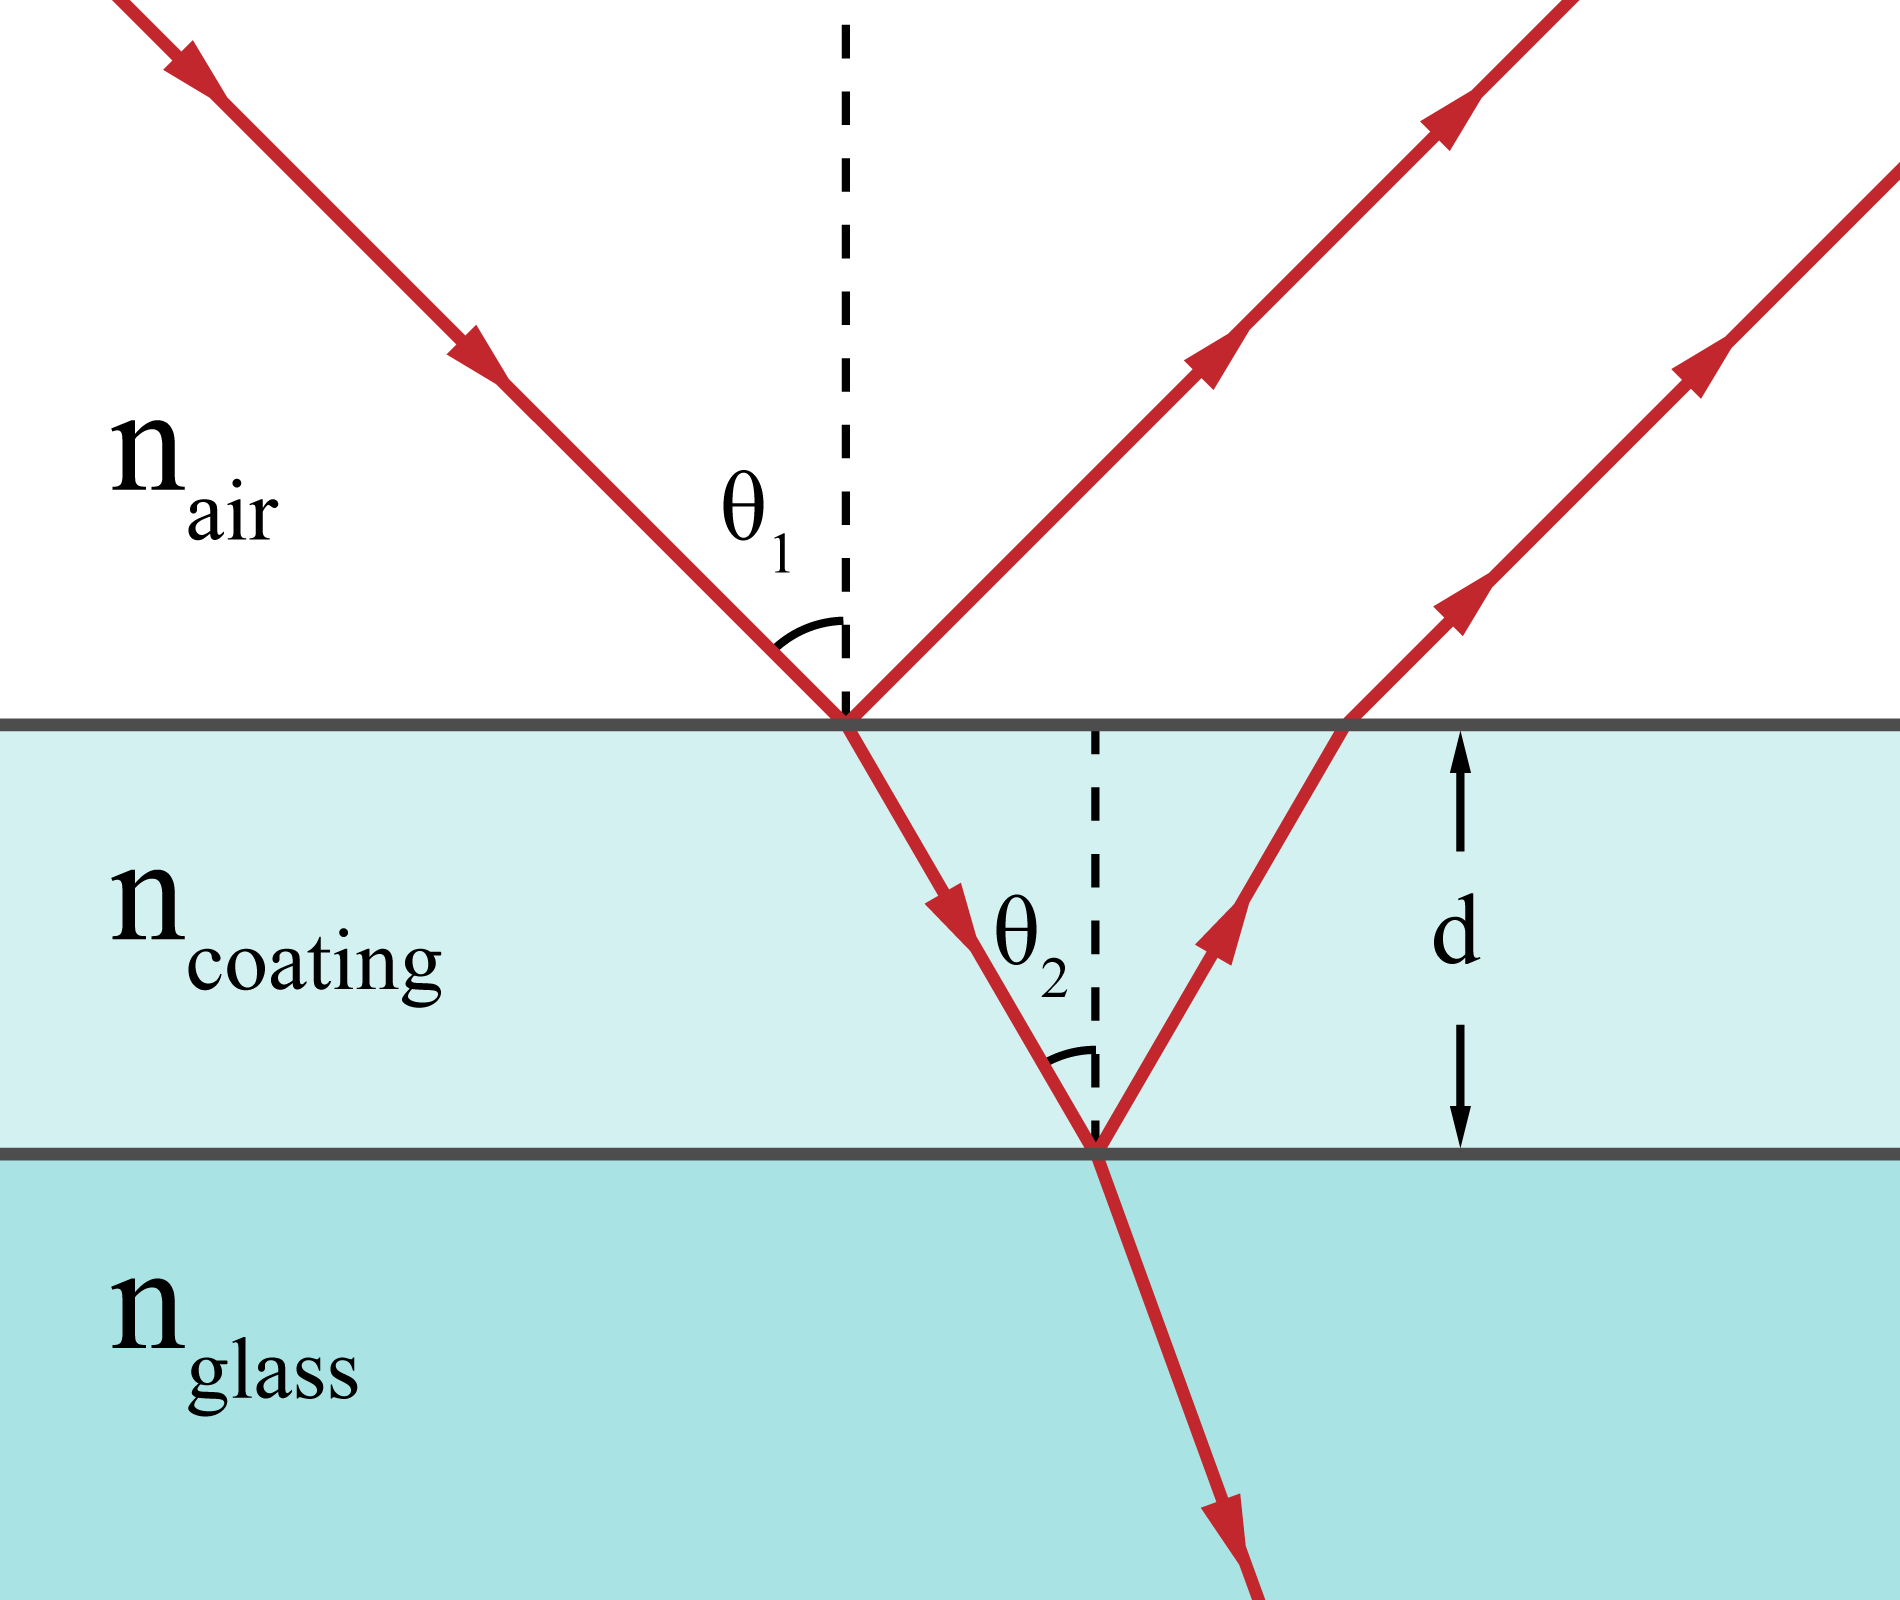
\includegraphics[width=55mm, height=40mm]{images/ThinFilmCoating.png}
      \tiny \url{https://en.wikipedia.org/wiki/Thin-film_interference}
      
      \large
      $n_{glass} > n_{film} >  n_{air}$
      
      Constructive: $2n_{coating}d \cos(\theta_2) = m \lambda$
      
      Destructive: $2n_{coating}d \cos(\theta_2) = (m-\frac{1}{2}) \lambda$
      
      
\end{minipage}

\\ \hline
}

\subsection{Diffraction}
\Table{
\hline

Single slit diffraction
&

\MiniPg{.7}{
\GraphicWHN{.55}{.4}{SingleSlit.png}
Fraunhofer Single Slit
\center
\tiny  \url{http://hyperphysics.phy-astr.gsu.edu/hbase/phyopt/imgpho/sinslit.gif}

}
 \\ \hline
}

\Table{
\hline

Double slit interference
&

\MiniPg{.7}{
\GraphicWHN{.8}{.5}{DoubleSlit.png}
\center
\tiny  \url{http://hyperphysics.phy-astr.gsu.edu/hbase/phyopt/imgpho/doubsli.gif}

\large 

}
 \\ \hline 
}

%%%%

\Table{
\hline

Diffraction grating
&

\MiniPg{.7}{
\GraphicWHN{.8}{.55}{Diffraction.png}
\center
\tiny  \url{http://hyperphysics.phy-astr.gsu.edu/hbase/phyopt/grating.html}

\large 

}

\\ \hline
}

%%%%

\Table{
\hline

Circular Aperture diffraction

&

\MiniPg{.7}{
\center

\GraphicWHN{.8}{.5}{ApertureDiff.png}
\center

Use for resolving power of telescopes.

\tiny \url{http://hyperphysics.phy-astr.gsu.edu/hbase/phyopt/cirapp2.html}

}

 \\ \hline 
}


%%%%%%%%%%%%%%%%%%%%%

\subsection{Geometrical  Optics}
\Table{
\hline

Optical Path Length & $OPL = \int_a^bn(s)\,ds$

\\ \hline
}

%%%%



%%%%%%%%%%%%


\subsubsection{Mirrors}

\center
\begin{tabular}{|p{5cm}|p{10cm}|}
\hline

For concave and convex spherical mirrors, the focal
length is & ... half the
radius of curvature of the mirror

\\ \hline
\end{tabular}

%%%%

\Table{
\hline
\MiniPg{.4}{
Spherical mirror eqn.
}

&

 \MiniPg{.6}{\center
$\dfrac{1}{f} = \dfrac{1}{d_O} + \dfrac{1}{d_i}$
}

\\ \hline

Spherical magnification & $M = \dfrac{h_i}{h_O} = -\dfrac{d_i}{d_O}$

 \\ \hline
}

%%%%

\Table{
\hline
 
 $d_O$ and object real/virtual & $d_O > 0 \rightarrow$ object in front (real). \\
 						& object in back (virtual) $\leftarrow d_O < 0$

\\ \hline
}

%%%%

\Table{
\hline

$d_i$ and image real/virtual & $d_i > 0 \rightarrow$ image in \textbf{front} (real). \\
 						& image in \textbf{back} (virtual) $\leftarrow d_i < 0$

\\ \hline
}

%%%%

\Table{
\hline

$f$ and concavexity & $f > 0 \rightarrow$ concave.convex $\leftarrow f<0$

\\ \hline

Magnification  image orientation & $M > 0 \rightarrow$ upright.inverted $\leftarrow M < 0$

\\ \hline
}


%%%%%%%%%%%%%%%%%%%%

\subsubsection{Lenses}

\Table{
\hline

\MiniPg{.3}{
Converging lens \_ mirror 

Relations for real, virtual, larger, smaller 
}
&
\MiniPg{.7}{
\center

 \begin{minipage}{.42\textwidth}
      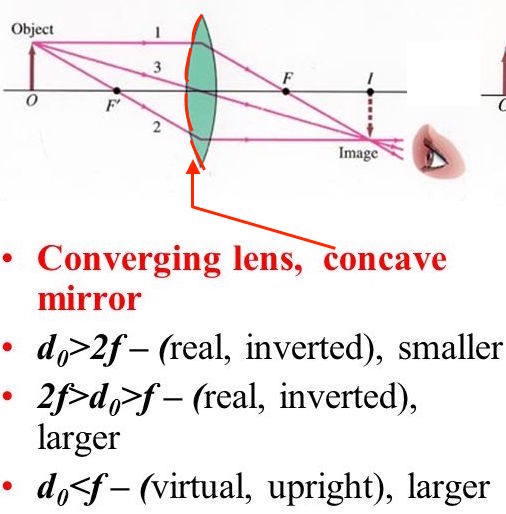
\includegraphics[width=\linewidth, height=50mm]{images/ConvLens.jpg}
       \end{minipage} 
} 

\\ \hline
}

%%%%

\Table{
\hline

\MiniPg{.3}{
Diverging lens \_ mirror 

Relations for real, virtual, larger, smaller 
}
&
\MiniPg{.7}{
\center

 \begin{minipage}{.42\textwidth}
      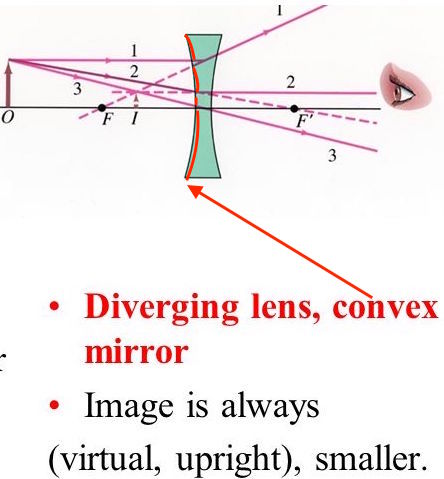
\includegraphics[width=\linewidth, height=50mm]{images/DivLens.jpg}
       \end{minipage} 
       
       \tiny \url{http://images.slideplayer.com/13/3858792/slides/slide\_13.jpg}
} 

\\ \hline

}

%%%%

\Table{
\hline

f-number or relative aperture & $\textrm{f-number} = N = \dfrac{f}{D} $ \\ 
					& where $f$ if focal length, $D$ is diameter
\\ \hline

Increased f & increased light-gathering power.

\\ \hline
}

%%%%

\Table{
\hline

Numerical aperture & $\textrm{n.a.} = n \sin \alpha$ \\

\begin{minipage}{.25\textwidth}
      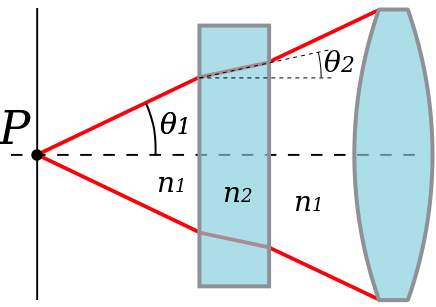
\includegraphics[width=\linewidth, height=32mm]{images/Numerical_aperture.png}
    \end{minipage} & \\
    \tiny https://en.wikipedia.org/wiki/Numerical\_aperture
     \large
    & 
    
    $\textrm{NA} = n_1 \sin \theta_1 = n_2 \sin \theta_2 $

\\ \hline
}

%%%%

\Table{
\hline

Relate NA to N (i.e. f-num) & \begin{minipage}{.25\textwidth}
      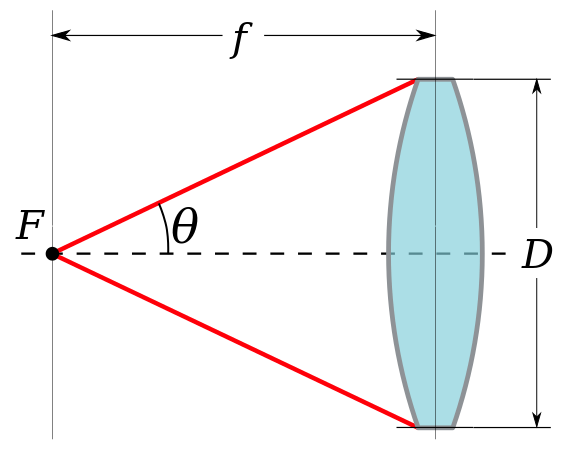
\includegraphics[width=\linewidth, height=30mm]{images/NA_fNum.png}
    \end{minipage} \\
    
     & $\textrm{NA}_i = n \sin \theta = n \sin [ \arctan \Big( \dfrac{D}{2f} \Big) ] \approx \dfrac{nD}{2f} $\\
     
      & $\Rightarrow N \approx \dfrac{1}{2 \textrm{NA}_i}$ assuming $n=1$.


\\ \hline
}

%%%%

\Table{
\hline

Formula for focal length (spherical) & $\dfrac{1}{f} = (n-1)\Big(\dfrac{1}{R_1} - \dfrac{1}{R_2} \Big),$ \\ 
& where $R_1$ is the radius of curvature for the lens \\
& nearest the object and $R_2$ is the r.o.c. for the farther

\\ \hline
}

%%%%

\Table{
\hline
\MiniPg{.4}{
Thin lens equation  (a.k.a. 'Lensmaker's formula') }

&

\MiniPg{.6}{\center
$\dfrac{1}{f} = \dfrac{1}{d_O} + \dfrac{1}{d_i}$
}

 \\ \hline
 
 $d_O$ and object real/virtual & $d_O > 0 \rightarrow$ object in front (real). \\
 						& object in back (virtual) $\leftarrow d_O < 0$

\\ \hline
}

%%%%

\Table{
\hline

$d_i$ and image real/virtual 
&

\MiniPg{.7}{\center
 $d_i > 0 \rightarrow$ image in \textbf{back} (real). 
 
 image in \textbf{front} (virtual) $\leftarrow d_i < 0$
 }
						
\\ \hline
}

%%%%

\Table{
\hline

$R_n$ and center of lens & $R_n > 0$ if center of lens in back \\
 						& $R_n < 0 $ if center of lens in front

\\ \hline
}

%%%%

\Table{
\hline

$f$ and concavexity & $f > 0 \rightarrow$ concave.convex $\leftarrow f<0$

\\ \hline

resulting $f$ for two close lenses & $\dfrac{1}{f} = \dfrac{1}{f_1} + \dfrac{1}{f_2}$

\\ \hline
}

%%%%

\Table{
\hline

Magnification & 

\MiniPg{.6}{
\GraphicWHN{.9}{.3}{LensMag.png}
\center
\tiny \url{http://hyperphysics.phy-astr.gsu.edu/hbase/geoopt/lensdet.html}
}

\\ \hline
}

%%%%

\Table{
\hline
\MiniPg{.3}{
Angular magnification of a telescope
}

&

\MiniPg{.7}{
\center
Astronomical telescope
\GraphicWHN{.85}{.3}{TelescopeAstro.png}

\center Galilean telescope
\GraphicWHN{.85}{.3}{TelescopeGali.png}
\center
For both: $M = -f_o/f_e$

}


\\ \hline
}


%%%%%%%%%%%%%%%%%%%%%%%%%%%%%%%%%%%%%%%%%%%


\subsection{Polarization}
\Table{
\hline

Malus' law & \begin{minipage}{.5\textwidth}
 First, consider electric field vector
 

$I_{transmitted} = I_0 \cos^2\theta_i$
\end{minipage}

\\ \hline

Intensity of polarized from unpolarized &  $I = I_0 \int_0^\pi \cos^2 \theta \, d \theta = \dfrac{I_0}{2}$

\\ \hline
}

%%%%

\Table{
\hline

Brewster's Angle 

&

\begin{minipage}{.7\textwidth}
\center

First, read Ch. 9 of Griffith's $EM$. It falls out of the Fresnel equations that there is 0 reflectance when

$\theta_1 + \theta_2 = 90^\circ$

Use Snell's law:

$n_1 \sin \theta_1 = n_2 \sin \theta_2$.

Let $\theta_B$ be the Brewster angle

$n_1 \sin \theta_B = n_2 \sin (90^\circ - \theta_B) = n_2 \cos \theta_B$,

Finally, $\boxed{\theta_B = \arctan\Big(\dfrac{n_2}{n_1}\Big)}$
 

\end{minipage}

\\ \hline
}

\Table{
\hline

Wire grid polarizer &  \begin{minipage}{.5\textwidth}
      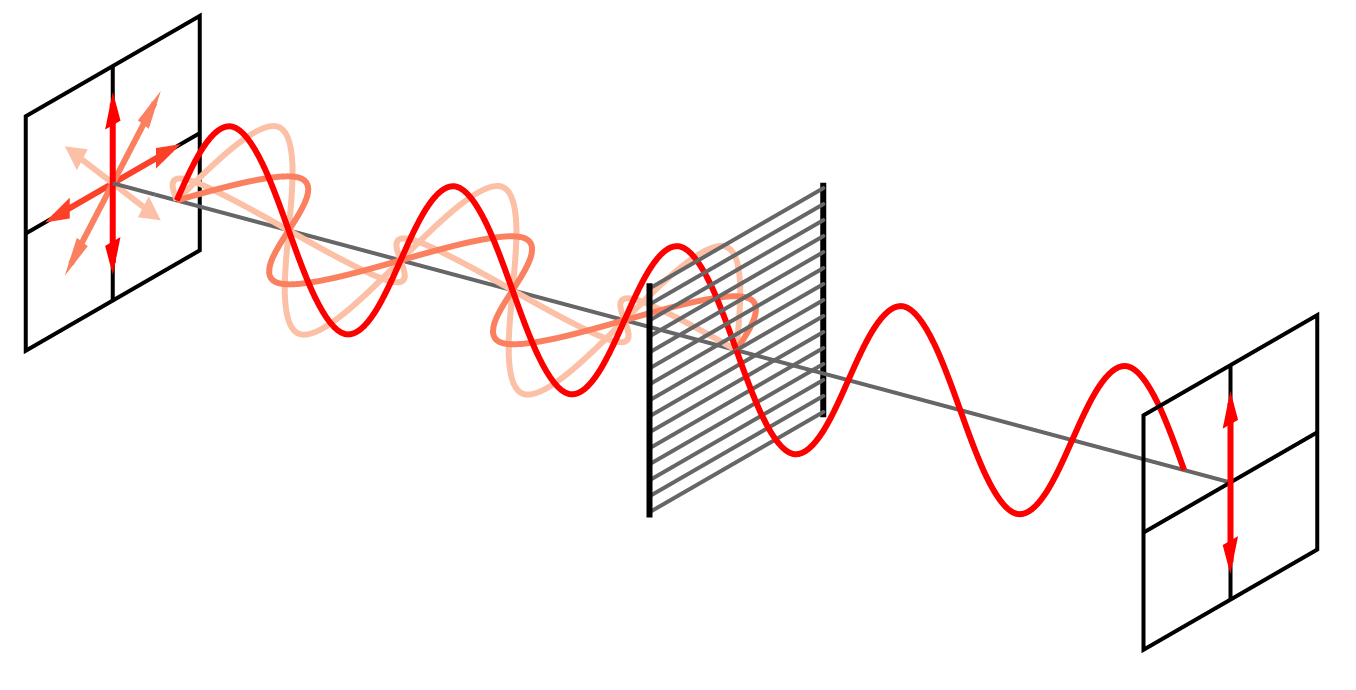
\includegraphics[width=\linewidth, height=45mm]{images/WireGridPolarizer.png}
      \tiny \url{https://en.wikipedia.org/wiki/Polarizer}
       \end{minipage}

\\ \hline
}

%%%%

\Table{
\hline

Polarized Sunglasses & \begin{minipage}{.5\textwidth}
      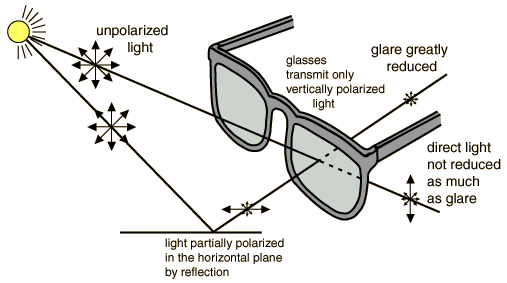
\includegraphics[width=\linewidth, height=45mm]{images/PolarizedSunglasses.png}
       \tiny \url{http://assets.openstudy.com/updates/attachments/4f175a76e4b0aeb795f5672a-jamesj-1326931194153-sunglass.gif}
       \end{minipage}
       
\\ \hline
}

%%%%

\Table{
\hline

$s$ and $p$ polarization & \begin{minipage}{.5\textwidth}
      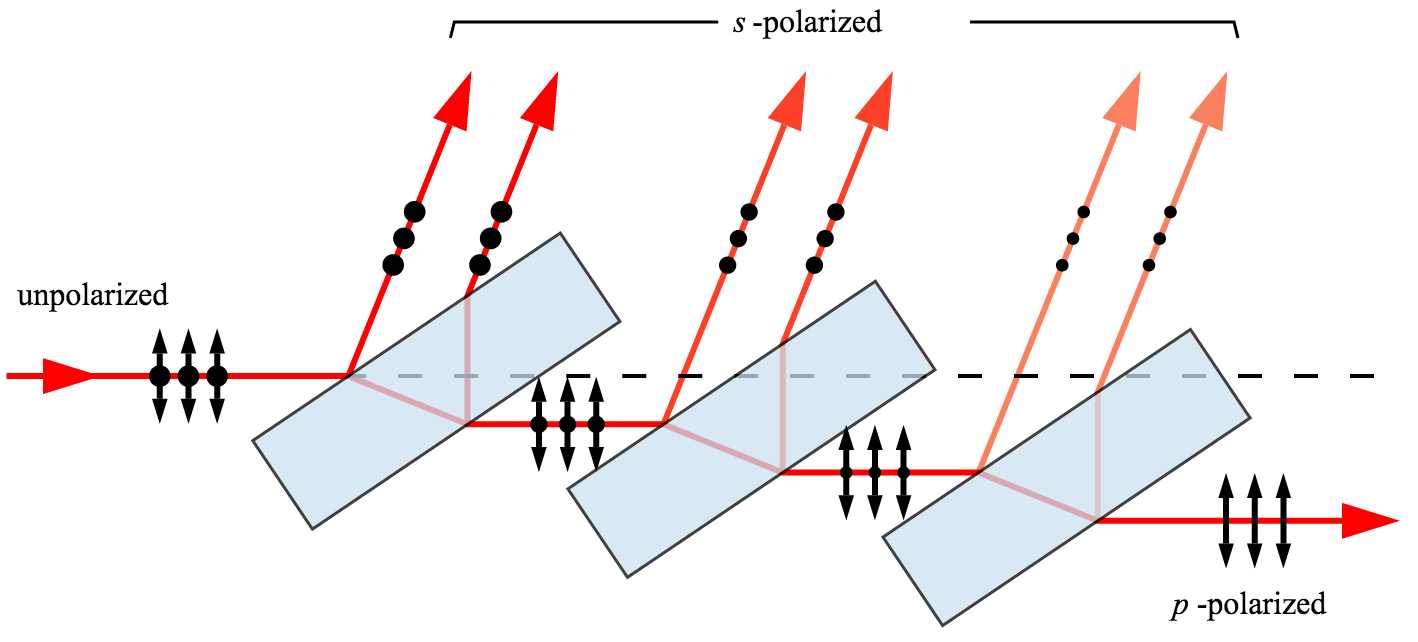
\includegraphics[width=\linewidth, height=35mm]{images/SandPpolarization.png}
      \tiny \url{https://en.wikipedia.org/wiki/Polarizer}
      
      \large Think `s' for ``smooth'' and `p' for ``pointy'' or ``points in.''
       \end{minipage}

\\ \hline
}

%%%%%%%%%%%%%%%%%%%%%%%%%%%%%%%%

\subsection{Doppler effect}
\Table{
\hline

Derivation 
Wavelengths& $c = $ velocity of waves in medium, \\
and & $v_s = $ velocity of source relative to medium, \\
Frequencies & $v_o = $ velocity of observer relative to medium. \\
& Waves travel from source to observer \\
& in the positive whatever direction: \\
& O....source)))))waves)))))observer......$>$+x \\
& Observer moving, source still: $c + v_o = \dfrac{\lambda_s}{T} $ \\
& Source moving, observer still: $c - v_s = \dfrac{\lambda_o}{T} $ \\
& $T = \dfrac{\lambda_o}{c - v_s} = \dfrac{\lambda_s}{c + v_o} $ \\
& \framebox{$\lambda_o = \dfrac{c - v_s}{c + v_o} \lambda_s$} \\
& \framebox{$f_o = \dfrac{c + v_o}{c - v_s} f_s $}

 \\ \hline
 }

